\documentclass[tikz,border=10pt]{standalone}
\begin{document}
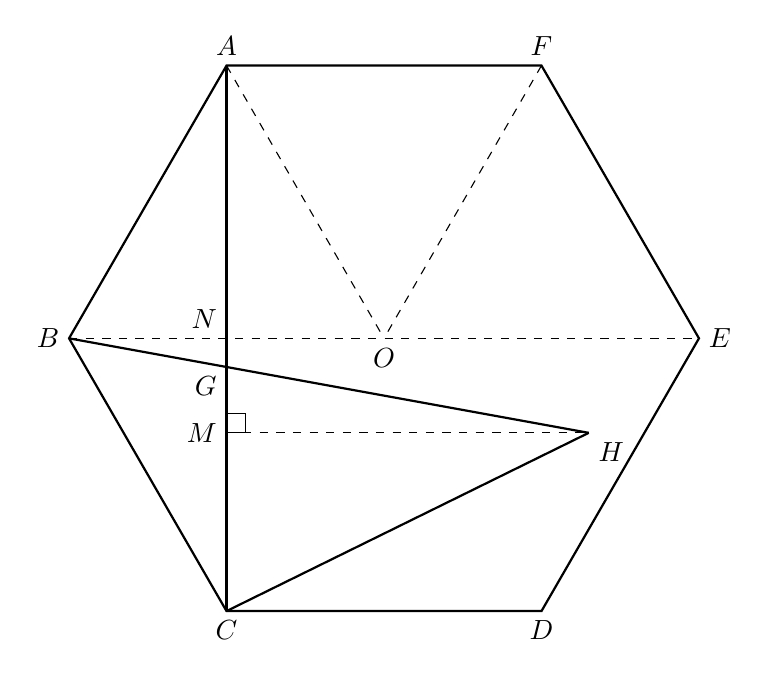
\begin{tikzpicture}[scale=2]
\coordinate (A) at (-1,1.732);
\coordinate (F) at (1,1.732);
\coordinate (B) at (-2,0);
\coordinate (E) at (2,0);
\coordinate (C) at (-1,-1.732);
\coordinate (D) at (1,-1.732);
\coordinate (O) at (0,0);
\coordinate (N) at (-1,0);
\coordinate (G) at (-1,-0.18);
\coordinate (M) at (-1,-0.6);
\coordinate (H) at (1.3,-0.6);

\draw[thick] (A) -- (F) -- (E) -- (D) -- (C) -- (B) -- cycle;
\draw[thick] (A) -- (C);
\draw[thick] (B) -- (H);
\draw[thick] (C) -- (H);
\draw[dashed] (B) -- (E);
\draw[dashed] (A) -- (O);
\draw[dashed] (F) -- (O);
\draw[dashed] (M) -- (H);

\draw (-1,-0.6) rectangle ++(0.12,0.12);

\node[above] at (A) {$A$};
\node[above] at (F) {$F$};
\node[left] at (B) {$B$};
\node[right] at (E) {$E$};
\node[below] at (C) {$C$};
\node[below] at (D) {$D$};
\node[below] at (O) {$O$};
\node[above left] at (N) {$N$};
\node[below left] at (G) {$G$};
\node[left] at (M) {$M$};
\node[below right] at (H) {$H$};
\end{tikzpicture}
\end{document}
